

\documentclass[12pt, final]{article}

%%%%%%%%%%%%%%%%%%%%%%%%%%%%%%%%%%%%%%%%%%%%%%%
\usepackage{virgil_env} %% Import the Virgil environment
%\usepackage{multirow}
%\usepackage{fullpage}
%\usepackage{nips10submit_e}
\usepackage{afterpage}
\usepackage{cite}
\usepackage{caption}
\usepackage{subfigure}
%\usepackage{subfig}

%\usepackage{subcaption}
%\nipsfinalcopy
%\input{this_symbols.tex}  %% symbols for this paper


\usepackage[utf8]{inputenc}


\graphicspath{{./}{figs/}}
% \usepackage{booktabs,nicefrac}

\usepackage{xspace}
\usepackage{float}


\usepackage{listings} % to make pretty code


% \usepackage{tabu}% http://ctan.org/pkg/tabu

\newcommand{\dashrule}[1][black]{%
  \color{#1}\rule[\dimexpr.5ex-.2pt]{4pt}{.4pt}\xleaders\hbox{\rule{4pt}{0pt}\rule[\dimexpr.5ex-.2pt]{4pt}{.4pt}}\hfill\kern0pt%
}
\newcommand{\rulecolor}[1]{%
  \def\CT@arc@{\color{#1}}%
}

%\newcommand{\tt}[1]{{\texttt{ #1 }}}
\newcommand{\fname}[1]{ \operatorname{ #1 } }
\newcommand{\opname}[1]{ \operatorname{ #1 } }
\newcommand{\opcode}[1]{\textsc{\texttt{#1}}}


%\usepackage{authblk}
\author{Virgil Griffith}
\author{???}
\author{Vitalik Buterin}
%\affil{Ethereum Foundation}
%\affil[2]{National University of Singapore}


%%%%%%%%%%%%%%%%%%%%%%%%%%%%%%%%%%%%%%%%%%%%%%%%%%%%%%%

\bibliographystyle{plos2009}

\usepackage{mathenv}
%\usepackage[]{algorithm2e}


\title{Blockchain Resource Pricing}

%%%%%%%%%%%%%%%%%%%%%%%%%%%%%%%%%%%%%%%%%%%%%%%%%%%%%%%%%%%%%%%%%%%%%%%%%%%%%%%%%%%%%%%%%%%%%%%%

%%%%%%%%%%%%%%%%%%%%%%%%%%%%%%%%%%%%%%%%%%%%%%%%%%%%%%%%%%%%%%%%%%%%%%%%%%%%%%%%%%%%%%%%%%%%%%%%


\begin{document}

\maketitle
\vspace{-0.2in} \TODO{\today}

%{\centering {\sffamily \today} \vskip10pt }

%\vspace{-0.2in} {\centering \today } \vspace{0.1in}



%\vspace{-0.05in}
\begin{abstract}
\todo{this will be reworked at the end} 

One of the most challenging issues in blockchain protocol design is how to limit and price the submission of transactions that get included into the chain. Every transaction confers some private benefit to its sender, but transactions also incur social costs to the network as a whole, as every node in the network must process every transaction. This results in a classic example of the ``tragedy of the commons'' problem. In such cases, economic theory generally dictates pricing the resources in question, and setting the price to equal the social cost that the act of consuming each resource imposes on the network. However, the heterogenous nature of the computation, bandwidth and storage resources involved, the large portion of the social cost that exists in the form of intangible and difficult-to-value harms such as centralization risk, and the need to create an automated algorithm that can set prices in a wide range of future scenarios without human intervention all make it very difficult to set restrictions that are optimal. In this paper, we discuss tradeoffs between different approaches and strategies that can improve on the status quo on the margin.
\end{abstract}

%%%%%%%%%%%%%%%%%%%%%%%%%%%%%%%%%%%%%%%%%%%%%%%%%%%%%%%%%%%%%%%%%%%%%%%%%%
\section{Introduction and Model}
%%%%%%%%%%%%%%%%%%%%%%%%%%%%%%%%%%%%%%%%%%%%%%%%%%%%%%%%%%%%%%%%%%%%%%%%%%

A blockchain is a decentralized network consisting of a large number of computers that must all process transactions that transaction senders upload to the chain. Hence, a transaction that is published to a blockchain confers some private benefit to its sender, but also confers an external social cost to the network's participants. In order to account for this social cost, and prevent abuse of the blockchain as a common pool resource, some economic mechanism for restricting what transactions get included is required. However, there are many types of economic mechanisms that can be used to solve resource pricing problems of this type, and understanding which one is optimal requires more deeply understanding the nature and types of social costs in question.

The social costs can be broken down in two ways. First, one can categorize by fundamental type of resource expenditure:

\begin{itemize}
\item[] \textbf{Bandwidth cost:} the cost of all nodes downloading each submitted transaction, bundling it into a block, and then rebroadcasting the transaction as part of some block.

\item[] \textbf{Computational cost:} the cost of every node verifying each transaction.

\item[] \textbf{History storage cost:} the cost of storing the transaction for all nodes that store the blockchain's history, for the time for which the history is stored (possibly infinity).

\item[] \textbf{State storage cost:} the marginal cost of the impact of the transaction on the size of the \emph{state} (eg. contract code, account balances) that every node must store to be able to process further transactions.
\end{itemize}

Note that the first two costs are costs that are paid by the nodes that are online at the exact time when the transaction is included, the third cost is paid by nodes that are online at that time or in the near future, but the fourth cost must be paid by all nodes forever, unless a scheme is introduced that makes all state entries temporary.

Second, one can categorize by different types of first and second-order effects. We can understand these effects as follows. We can consider a blockchain to be a network of $n$ computers, $C_1 ... C_n$, where any transaction that gets included in the blockchain must be processed by all of the nodes that are still online in the network. Some transactions are more complex than others; each transaction has some ``weight'' $W$ that represents the quantity of resources needed to process it.

Each user $U_i$ has some direct resource cost function $R_i(W)$ representing the cost to the user of processing a given amount of weight. This cost can include electricity and bandwidth costs, marginal disk wear and tear, inconvenience from a user's other applications running more slowly, reduced battery life, and so on. For sufficiently high $w$, at some point the costs become unacceptable to any given user, at which point the user will drop offline (we assume $R_i(W)$ is flat above this point). Let $NodeCount(W)$ be the number of users still online at weight $W$. Note that different users could drop offline at different points for either of two reasons: (i) some users have a lower resource cost than others, and (ii) some users value being connected to the blockchain more than others.

There is some utility function $D(k)$ reflecting the social value of the level of decentralization achieved by having the number of online nodes, which can be translated into a function $D(W)$ of the total transaction load. There may also be some cost function $A(W)$ that reflects the increased attackability of the network as more transactions get included. We can summarize all of these costs as a combined cost function $C(W) = \sum_i R_i(W) + (A(W) - A(0)) - (D(W) - D(0))$.

The above suffices as a model of a blockchain for the purpose of this paper; we do not need to care about details about proof of work, proof of stake, block structure, etc, except insofar as the details of those consensus algorithms and blockchain design patterns affect $NodeCount$ and $A$, and therefore $C$.

\section{Prior Work}

In Bitcoin and Ethereum, resources are priced using a simple ``cap-and-trade'' scheme. A metric is defined for the quantity of resources (called ``weight'' or ``gas'') that a transaction consumes, and there is a protocol-defined maximum total quantity of resources that the transactions contained in a block will consume. Validators have free rein to select transactions as long as the total weight of the block is below that limit. An equilibrium is established where users attach fees to their transactions which go to the validator that includes the transaction in a block, and validators select the transactions paying the highest fee per unit weight. In Bitcoin, for example, the weight limit is a static $4 *10^6$, and weight is defined as follows\cite{weightunits}:

\begin{scriptsize}
\begin{equation}
\tt{weight(block) = 4 * len(block.nonsignature\_data) + len(block.signature\_data)}
\end{equation}
\end{scriptsize}

Where $len(x)$ returns the number of bytes in $x$. For technical reasons that have to do with attempting to price in history and state storage costs, the bytes in signatures of transactions are priced more cheaply than the non-signature data in transactions. In Ethereum, there is a measure called ``gas'' which incorporates the size of the block as well as the computational cost of verifying transactions and executing smart contract code. For simplicity of exposition, this can be approximated as:

\begin{footnotesize}
\begin{equation}
\tt{weight(block) = 68 * len(block) + 3 * num\_computational\_steps\_in\_block}
\end{equation}
\end{footnotesize}

The gas function is in reality much more complex, but similar in spirit. There is a per-block gas limit, which validators can vote on (when creating a block, a miner can ``upvote'' or ``downvote'' the gas limit by a maximum of $\sim\!0.1\%$), and at the time of this writing most validators are voting for a gas limit of $\sim \! 8$ million.

A major problem with this approach is that a priori it has been difficult to determine a reasonable weight limit, and the question has often been a source of controversy\cite{blocksizedebate}. The purpose of this paper will be to try to go beyond the one-dimensional design space of ``there must be some limit, what should it be?'' and explore a much larger space of policies that attempt to address transaction resource consumption externalities, and try to develop policies that are both closer to optimal at the present time, and more robust to changes in economic circumstances in the long-term future, reducing the need for ``extra-protocol interventions'' such as hard forks.

\section{Pricing Resources under Uncertainty}
\label{sect:uncertainty}
Blockchain resource pricing has many parallels to regulatory responses to environmental pollution.  Particularly, although the validator of a block is compensated for publishing the transactions, the cost of that block being published is borne by \emph{all full nodes}, much like how pollution produced by one factory must be suffered by everyone living in the village (if not an even larger area).  This cost being borne by all full nodes is the negative externality that we wish to limit.  Both blockchains and environmental regulators use economic interventions to limit activities with negative externalities, where the negative externalities have both measurable components as well as components with high Knightian uncertainty (i.e., ``unknown unknowns'') \cite{knight1921risk}.  Many results from environmental economics \cite{barder14} are directly applicable to blockchains.

Weitzman's 1974 paper ``Prices vs Quantities'' \cite{weitzman1974prices}, outlines the tradeoffs between regulation by price (e.g., carbon taxes) versus regulation by quantity (e.g., issuing a fixed number of permits and letting them trade on the market). One important insight that Weitzman cites is that if the policymaker has perfect information about the social cost function and the demand curve for consuming the resource (a.k.a. the ``benefit function''), the two approaches are equivalent: for any desired price, one can choose an equivalent quantity-based policy by issuing exactly the number of permits equal to the equilibrium quantity that would be purchased at that price. However, when there is uncertainty about the position and shape of the cost-benefit curves, the two approaches have substantial differences.

Consider a world where the marginal social cost (negative externalities) of consuming a resource is fixed, but the marginal benefit function is rapidly decreasing. If a policymaker sets a quantity limit that is too low, then the quantity limit will intersect the marginal benefit curve at a point where the cost and benefit are much higher than the social cost, and consumers suffer very large opportunity costs from nonconsumption.  But if a policymaker instead sets a price, then the damage from a miscalculation is much lower.

If on the other hand, the \emph{private} cost of abstaining is fixed yet the marginal social cost of consumption increases rapidly, then setting a price is riskier. For example, consider a scenario where the social cost of consuming $<1,000$ resource units is acceptable, but going above 1,000 risks disastrous consequences (e.g., some ``tipping point'' theories of global warming\cite{wiki:runaway}). The marginal social cost of consuming an additional resource unit in a world where people are already consuming 1,050 resource units will be much higher than the marginal social cost in a world where people are merely consuming 900. In this case, if a policymaker anticipates a consumption of 900, and targets a tax to equal the marginal social cost at the 900 level, then the policy will be massively underpricing the additional social harm caused by additional resource consumption. On the other hand, a policymaker that simply issues 900 permits and allows them to trade on the market would see the risk mitigated.

\begin{center}
%\subfigure[]{
	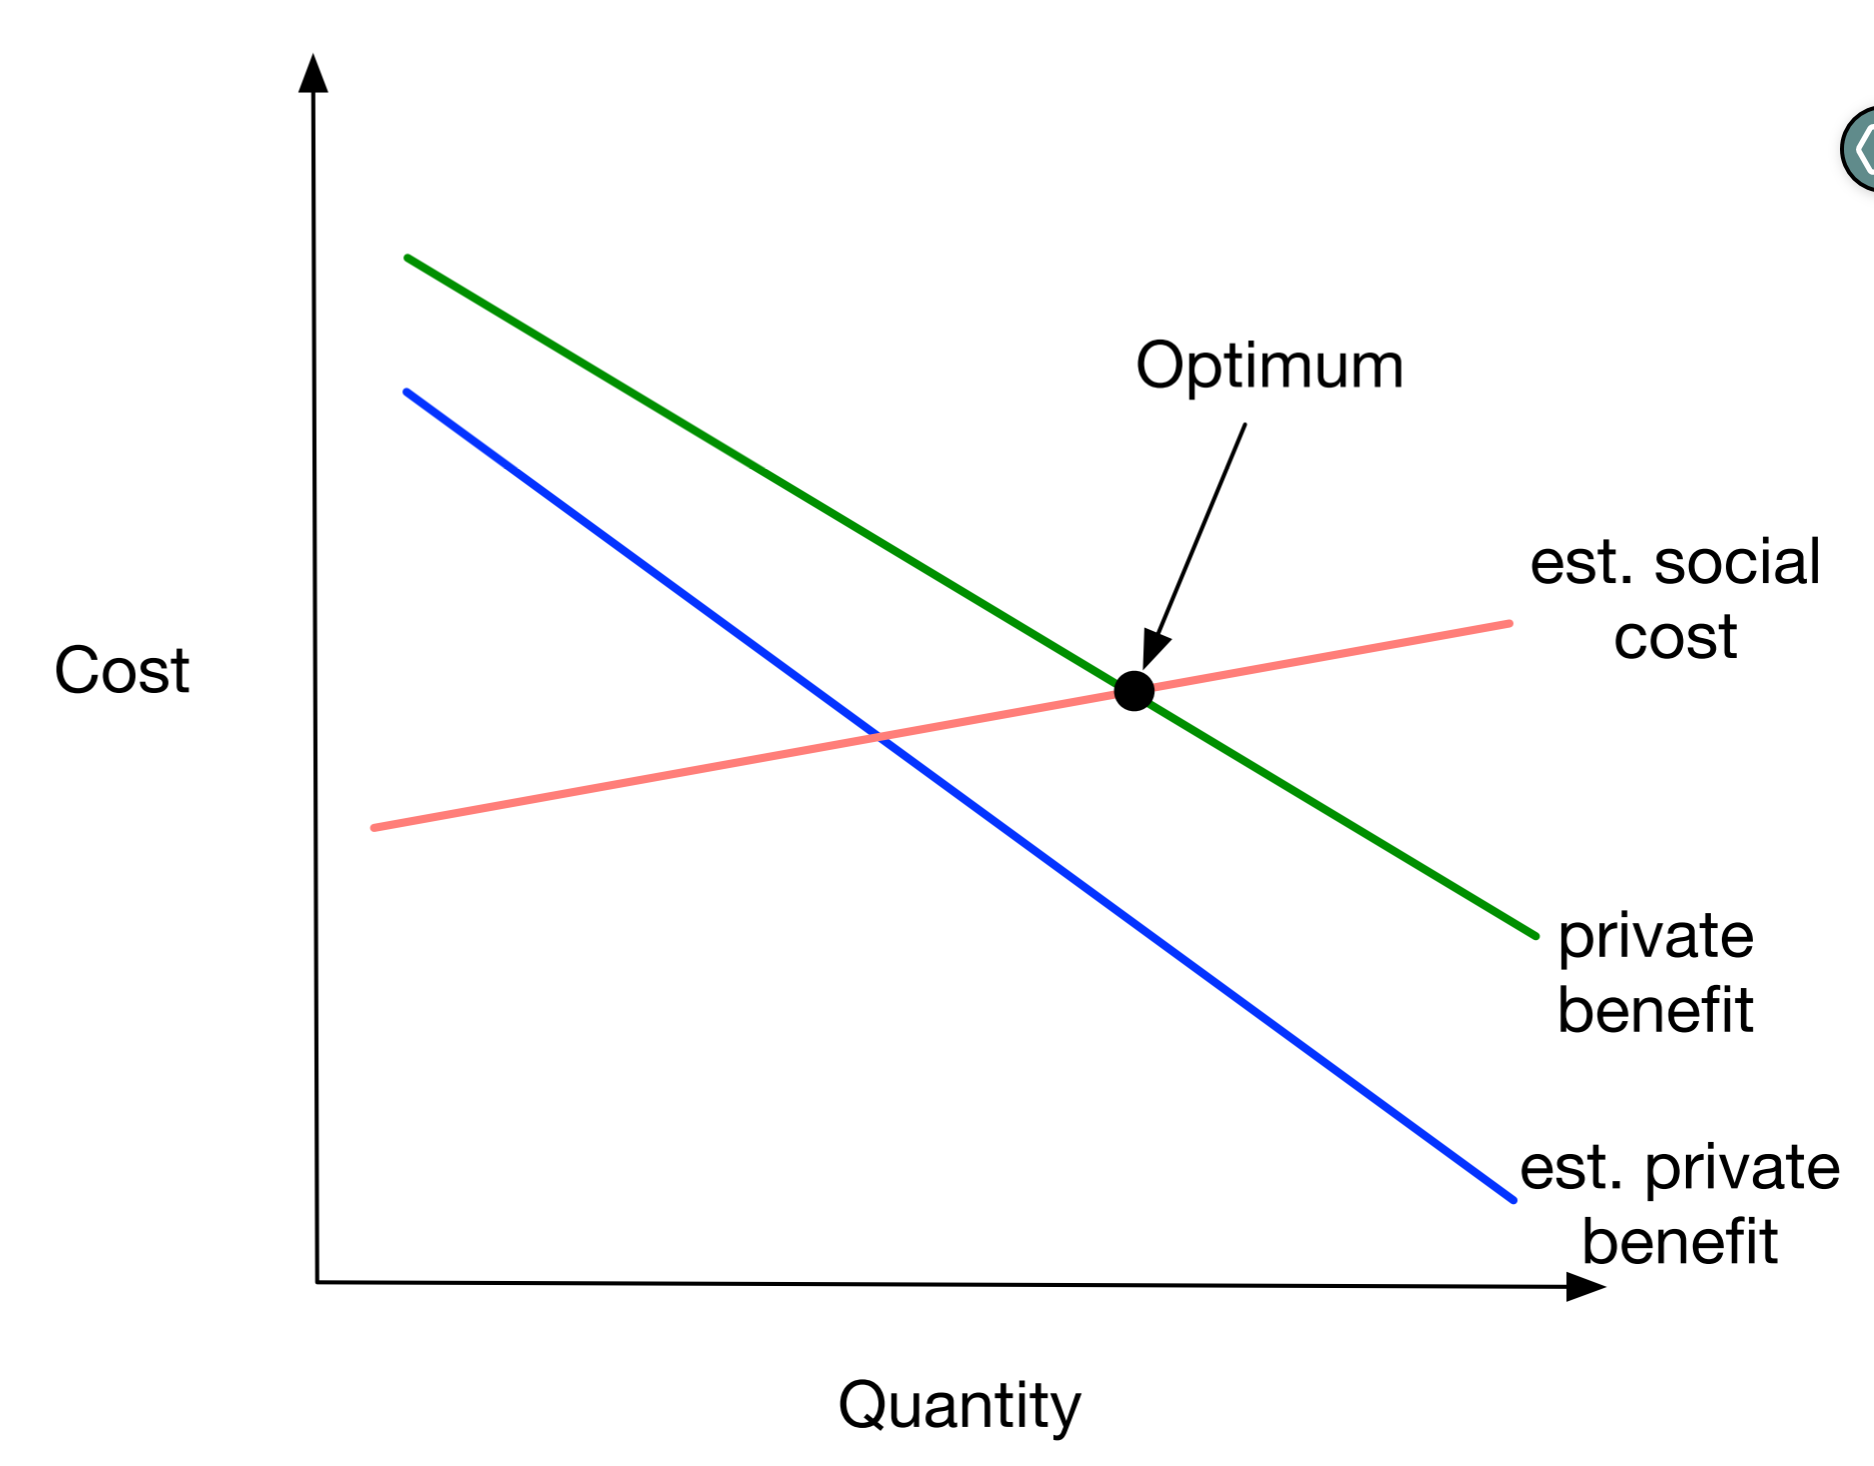
\includegraphics[width=2.25in]{fig1a.pdf}
%    \label{fig:1a}
%}
%\subfigure[]{
	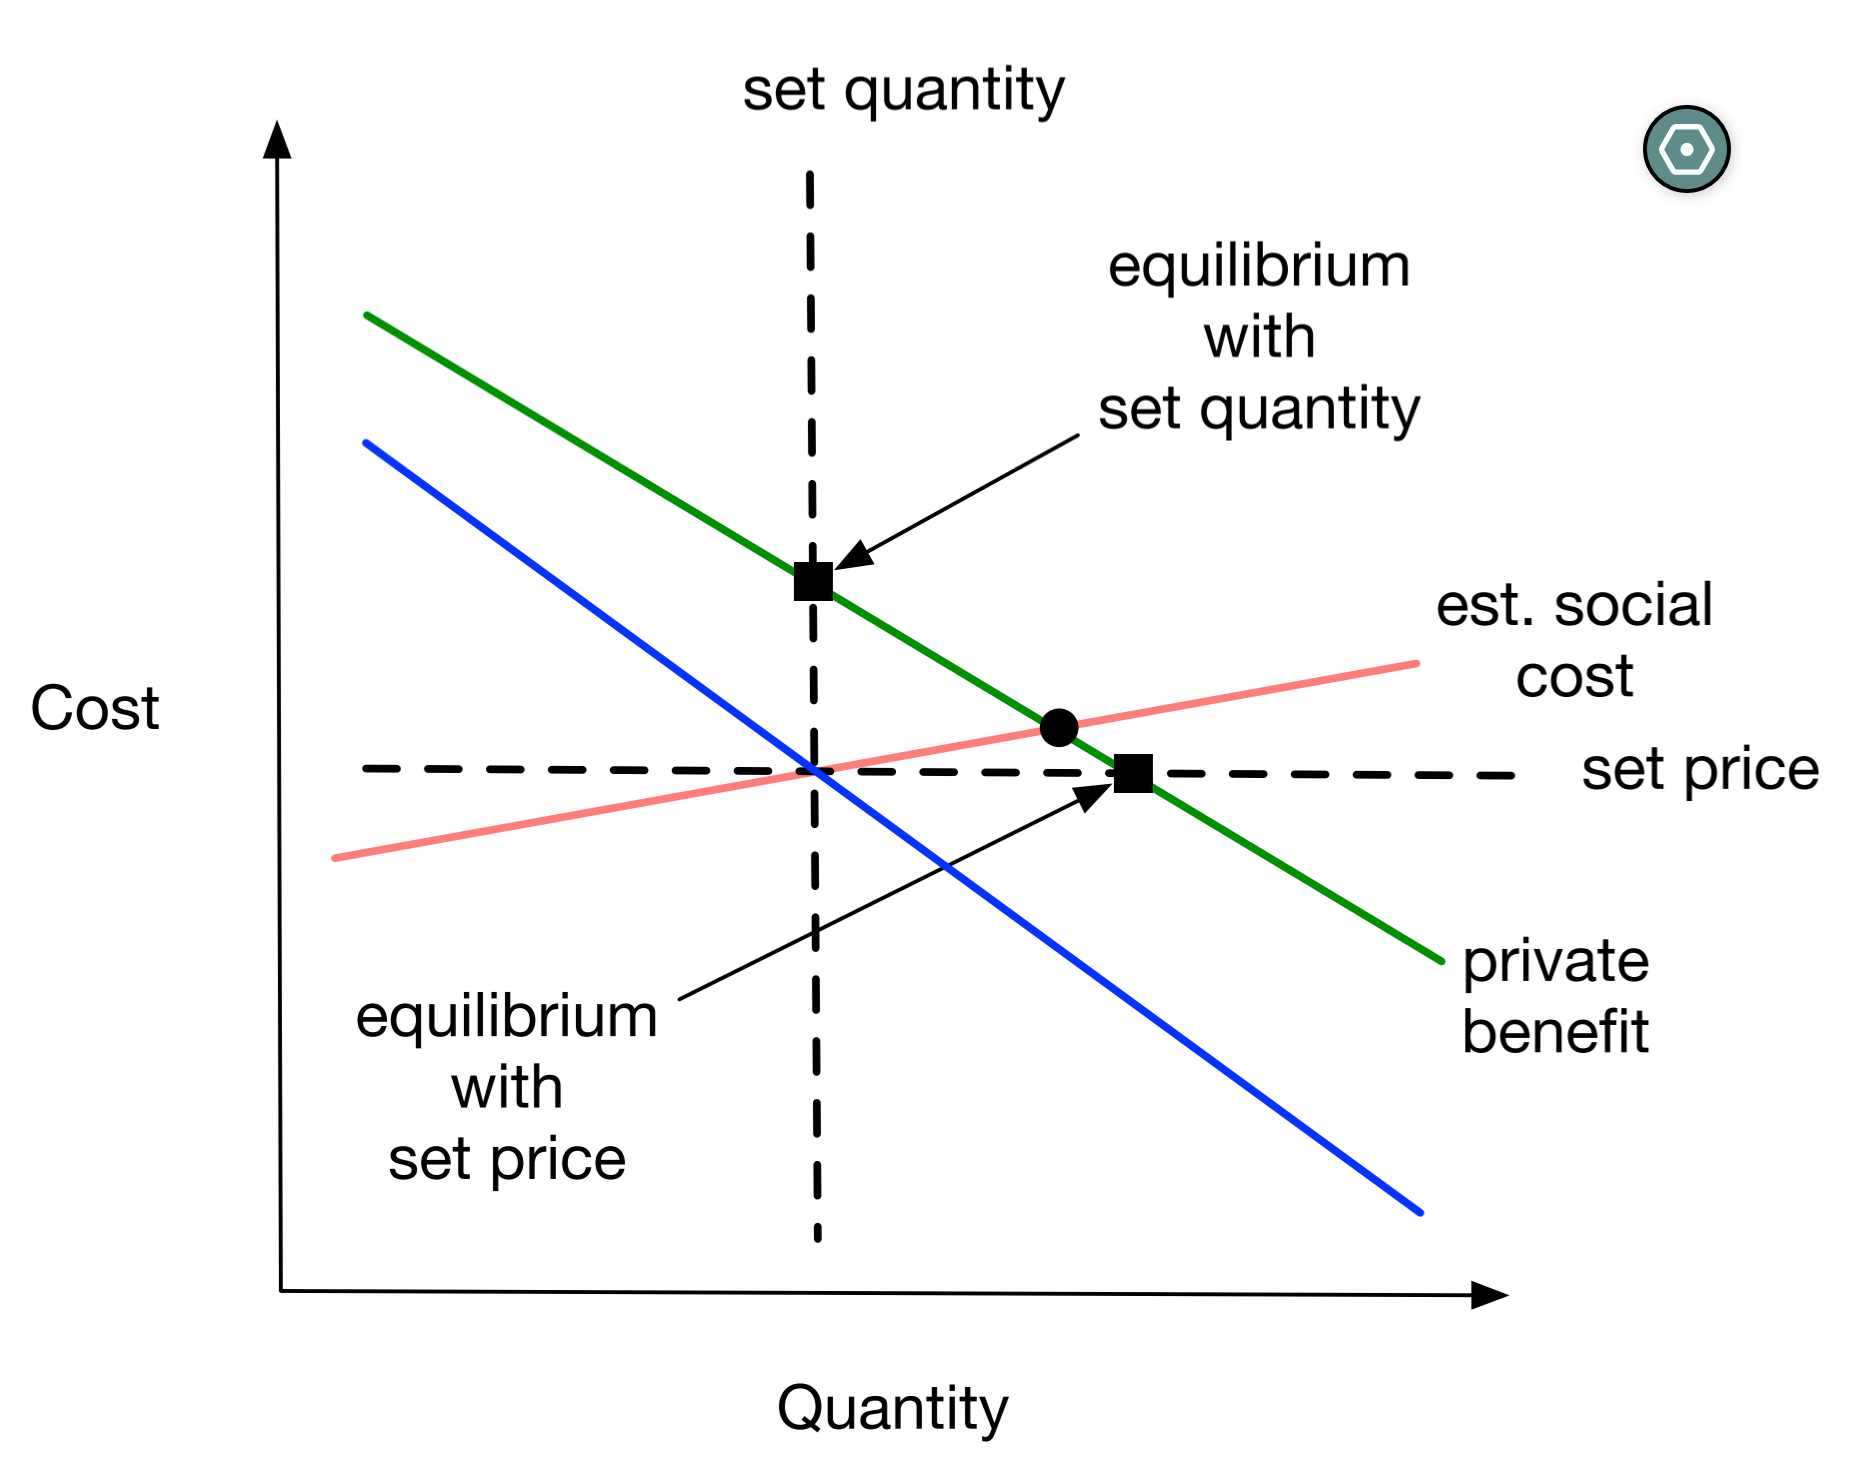
\includegraphics[width=2.25in]{fig1b.pdf} \\
%    \label{fig:1b}
%}

%\subfigure[]{
	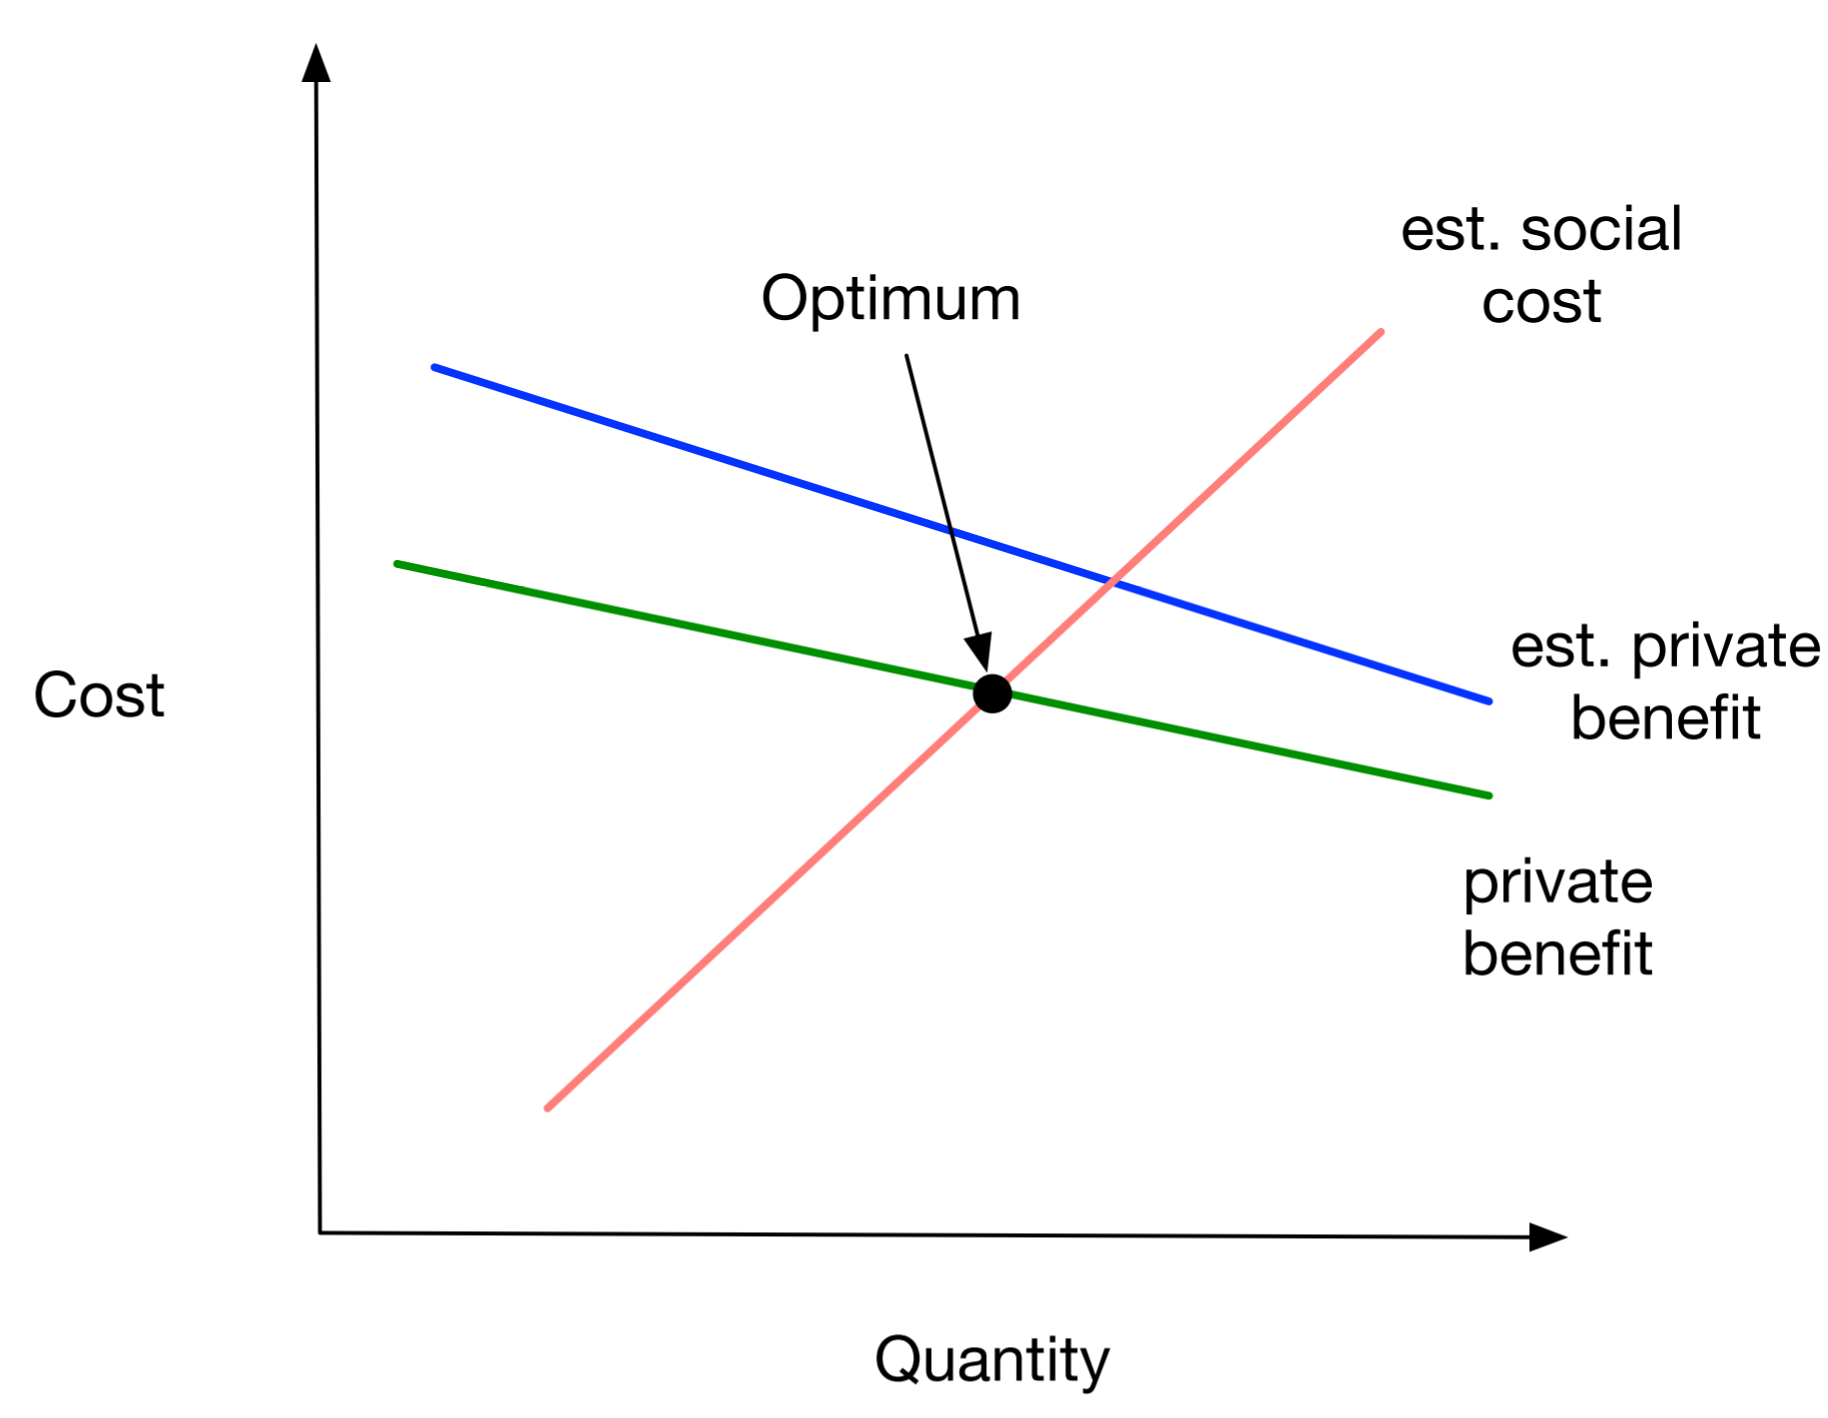
\includegraphics[width=2.25in]{fig1c.pdf}
%    \label{fig:1c}
%}
%\subfigure[]{
	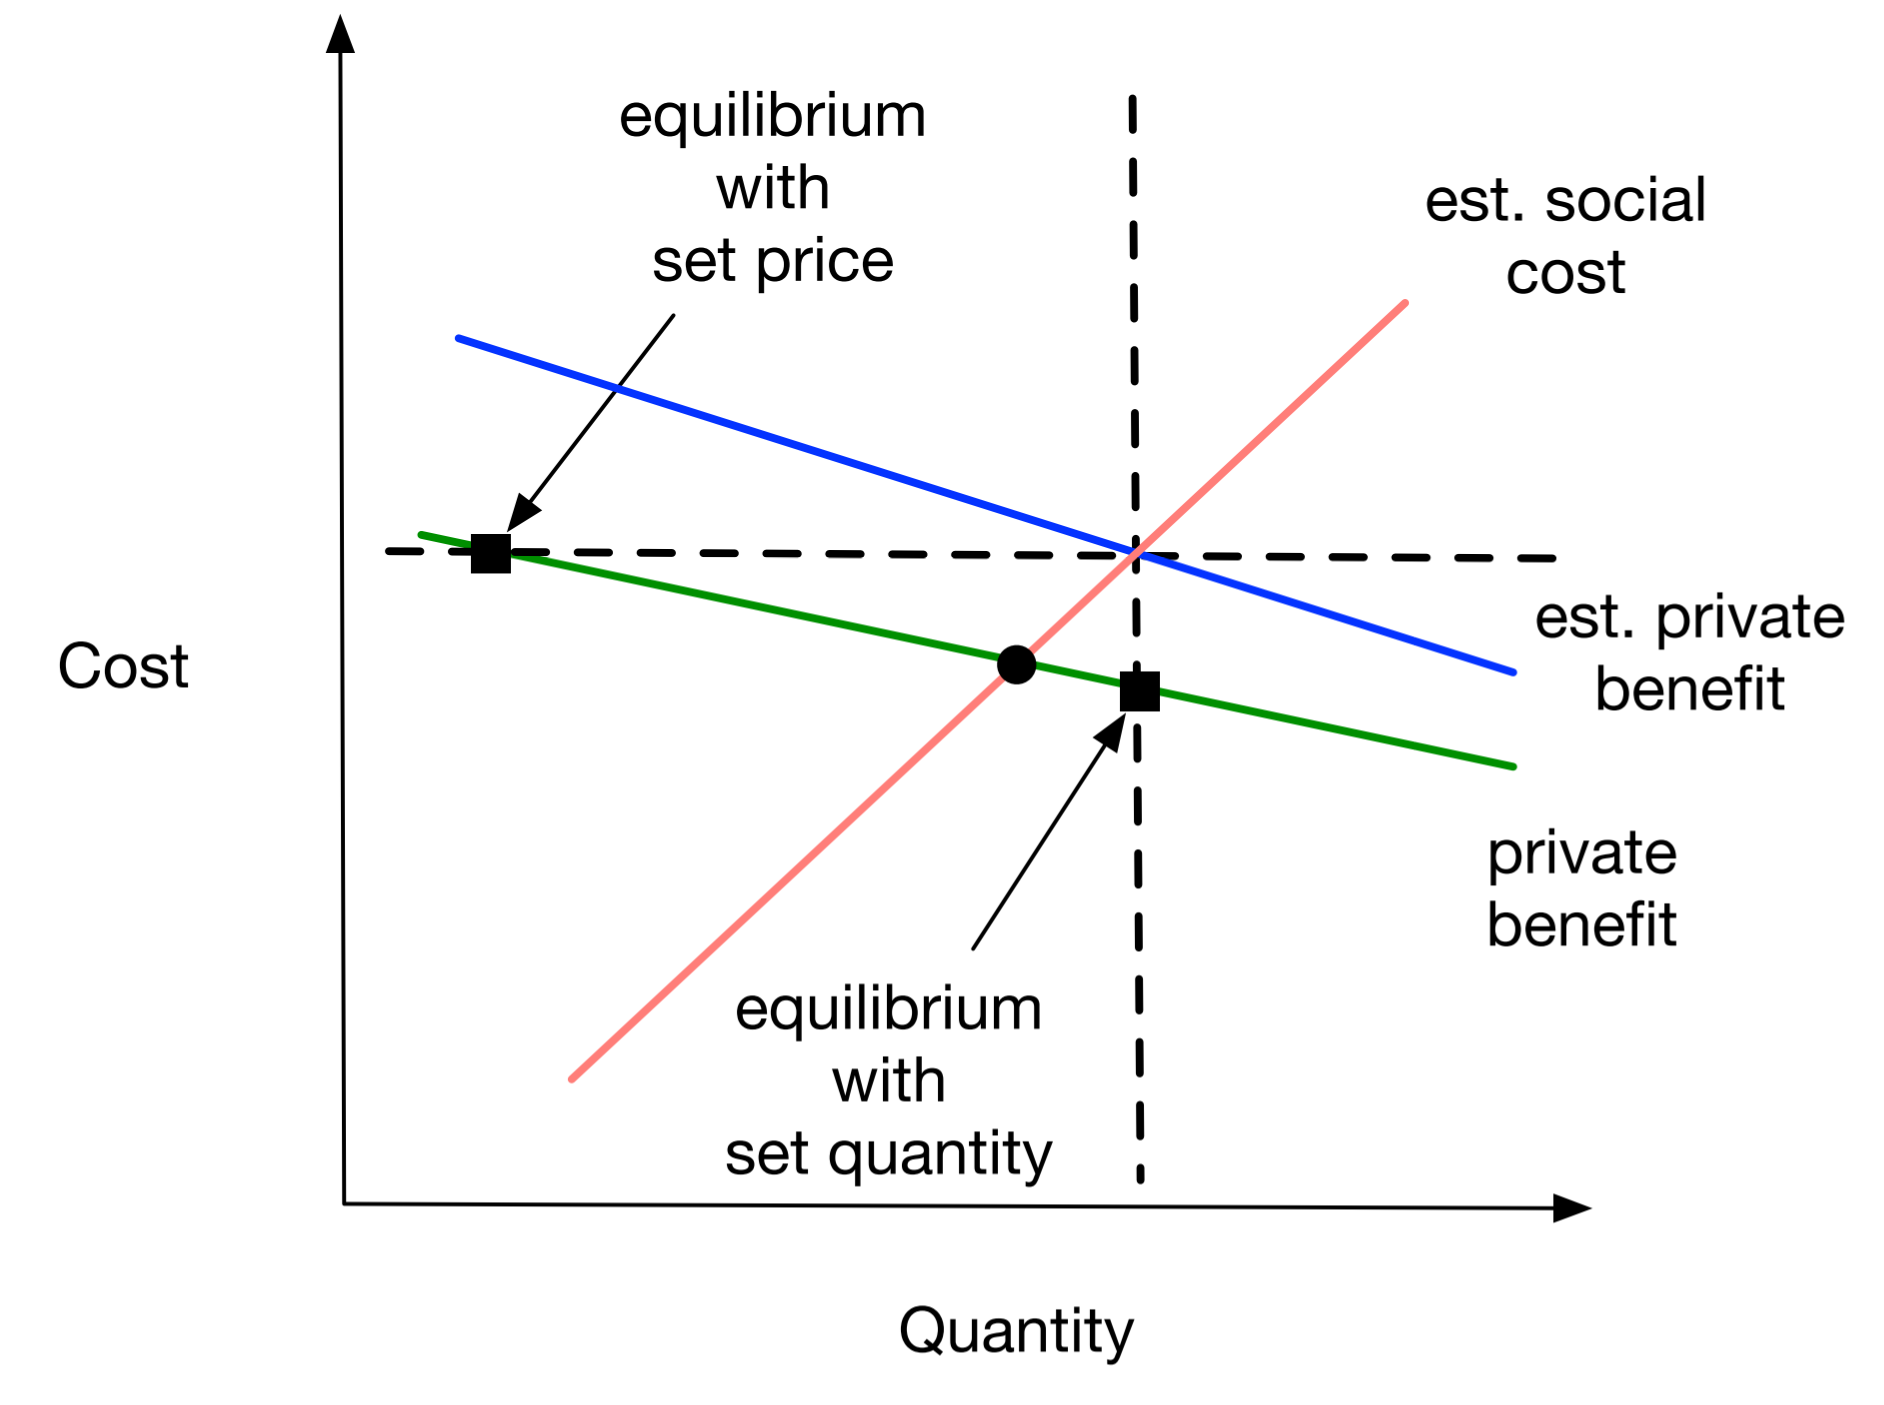
\includegraphics[width=2.25in]{fig1d.pdf} \\
%    \label{fig:1c}
%}
%\caption{Figures (a)--(b) show the first scenario in which it's better to set a price.  Figures (c)--(d) show the second scenario where it's better to set a quantity.}
Figures (a)--(b) show the first scenario in which it's better to set a price.  Figures (c)--(d) show the second scenario where it's better to set a quantity.
\label{fig:one}
\end{center}

Taken together, if the consumer's marginal private costs increase faster with quantity than the marginal social costs, that is when

\begin{equation}
\frac{ \fname{private\_benefit}^{\prime \prime}( \opname{quantity} ) }{ \fname{social\_cost}^{\prime \prime}( \opname{quantity}) }  > 1 \; ,
\end{equation}

then seting prices is better, and in other cases setting quantities is better.  Note that we need to use the second derivative because we are specifically talking about the \emph{the rate of change in marginal costs}.

The argument above applies only if costs and benefits are independently distributed. If changes in the cost and benefit curves are correlated, then an additional term must be added into the choice rule, increasing the relative attractiveness of limiting quantity. To see this intuitively, consider the extreme case where uncertainty in cost and benefit is perfectly correlated; in such a scenario, if original estimates of cost and benefit prove incorrect, both curves will move up or down in lockstep, and so the new equilibrium will be directly above or below the original estimated one; hence, a quantity-targeting policy would be perfectly correct and a price-targeting policy would be pessimal. This analysis covers only two possible policies, but a much greater space of options is available.  One can think of policy space as the space of possible supply curves for a given resource, where a pricing policy represents a horizontal supply curve and a cap-and-trade scheme represents a vertical supply curve. Various forms of diagonal supply curves are also possible, and in most cases some form of not strictly horizontal or vertical supply curve is optimal.

Should blockchains have a block size limit, or should they not have a limit but instead charge a fixed fee per resource unit consumed, or would some intermediate policy, one which charges a fee as a function $F(w)$ of the weight included in a block and where $F'(w)$ is increasing and possibly reaches an asymptote, be optimal? To estimate optimal policy under the prices vs. quantities framework, we start off by attempting to estimate the social cost function.

A study from Cornell\cite{cornell} provided an estimate of the node count as a response to the weight load of the blockchain. The study was conducted at a time when Bitcoin's weight formula was simply one weight unit per byte, with a weight limit of $10^6$. The study found that 90\% of nodes would remain online at $W = 4*10^6$, and 50\% of nodes would stay online at $W = 3.8 * 10^7$.

%\begin{figure}
	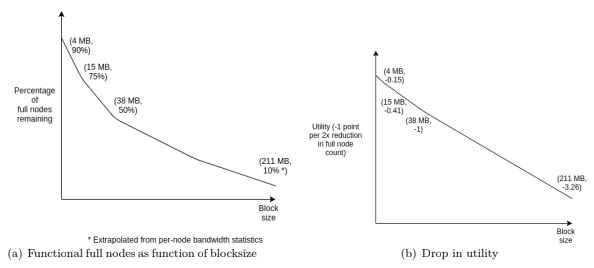
\includegraphics[width=5.5in]{blocksize_fullnodes.png}
%\end{figure}

%    \label{fig:1a}
    %\caption{Functional full nodes as function of blocksize from \cite{cornell-position}}

As a first approximation to quantifying the value to decentralization from having more nodes, we can use a logarithmic utility: $D(W) = log(NodeCount(W))$. What we discover is that $NodeCount(W)$ is roughly proportional to $\frac{1}{W}$, which in turn implies that $D(W) = -log(W)$. This in turn implies $D'(W) = \frac{1}{W}$: the marginal social cost function is \emph{decreasing}.

However, this model fails to take into account other kinds of harms that come as a result of large blocks taking a longer time to propagate. A study by Decker and Wattenhofer in 2013 found that the time that it takes for a block to propagate through the network is roughly linear in the block's size. Zohar and Sompolinsky\cite{GHOST} show that with a network delay $t$ and block time $T$, the rate of honest block creation slows from $\frac{1}{T}$ to $\frac{1}{T+t}$, reducing resistance to ``51\% attacks'' from $\frac{1}{2}$ to $q$ where $\frac{q}{1-q} * \frac{1}{T} = \frac{1}{T+t}$, i.e. $q = \frac{T}{2T + t}$. It seems reasonable to define a cost function $A(x) = \frac{1}{MinAttack(x)}$, where $MinAttack(x)$ is the minimum size of an attack that can succeed; since $MinAttack(x) = \frac{T}{2T + t}$, this implies that $A(x) = 2 + \frac{t}{T}$. $t$ is a function of $W$; if $t$ is linear in $W$, then that implies that $A(W) = 2 + k * W$ for some constant $k$, so the social cost function is linear.

In the case of Ethereum, we can try to look at the correlation between block gas usage and the ``uncle rate'', a measure of the percentage of blocks produced that do not make it into the canonical chain and hence that do not contribute to chain security.

\begin{center}
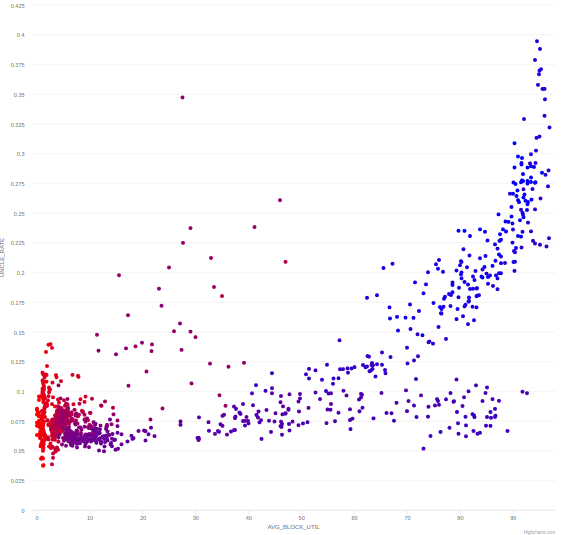
\includegraphics[width=3in]{etherchain_correlation.png} \\
\footnotesize{Relationship between block gas limit and uncle rate}
\label{fig:three}
\end{center}

The nonlinearity in this figure is in part an artefact of the data; during the period in late 2017, the composition of transactions changed away from smart contract use cases toward ERC20 token transfers, which affect uncle rate more than smart contract uses as their gas consumption is largely from bandwidth and computation costs and not code and storage. The dots at the top left are the 2016 DoS attack. Here's the same graph rescaled with the dots from late 2017 and the 2016 DoS attacks removed:

\begin{center}
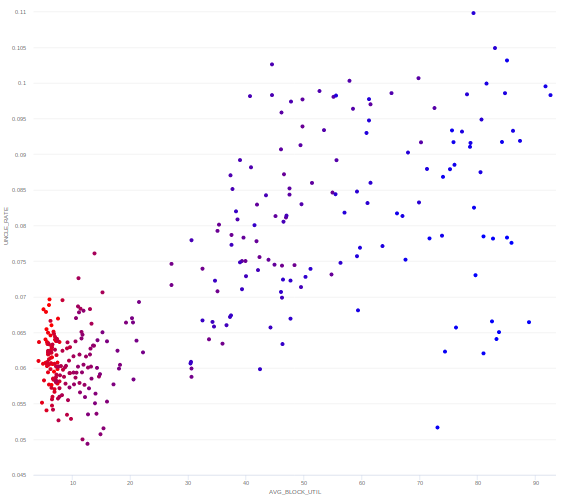
\includegraphics[width=3in]{etherchain_correlation_2.png} \\
\footnotesize{Relationship between block gas limit and uncle rate, Dec 2016 to Sep 2017}
\label{fig:three}
\end{center}

However, there are superlinear costs at play as well. Clients need to process both the main chain and the blocks that do not become part of the canonical chain; hence, if a level of canonical-chain throughput $x$ causes an uncle rate $p$, then the actual level of computational burden is $\frac{x}{1-p}$, with a denominator that keeps decreasing toward zero as the canonical-chain throughput increases. Additionally, with high uncle rates selfish mining attacks become much easier \cite{optimalsm}, and the reduction in node count itself leads to pooling, which makes selfish mining more likely. There is thus a qualitative sense in which the social cost of increasing $W$ to whe point where $t = T$ is more than ten times that of setting $W$ so that $t = T * 0.1$.

Even if the cost function is superlinear at the extremes, however, it appears to be linear at the lower side of the distribution, and the arguments from the Cornell study suggest it may even be sublinear. If the block size increases from 10kb to 1000kb, a significant social cost is incurred because IoT devices, smartphones, Raspberry Pis, etc have a much harder time staying connected, but an increase from 1000kb to 1990k does not have such a high cost, because the range of use cases that become unusable within that interval is much lower. Hence, it seems plausible that the social cost curve is U-shaped:

\begin{center}
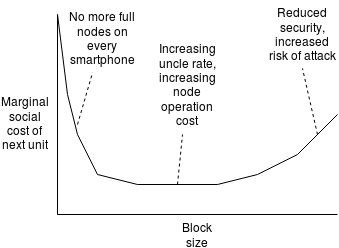
\includegraphics[width=3in]{total_social_cost.png} \\
\footnotesize{Rendering of a possible total social cost curve for blockchains accepting transactions}
\label{fig:three}
\end{center}

\subsection{Estimating the Private Benefit Curve}

The private benefit curve, the demand for sending transactions, is much harder to estimate. We will try to make some estimates of a single variable, the elasticity of demand (ie. by what percent demand increases with a 1\% fall in price), by looking at some ``natural experiments'' in the Bitcoin and Ethereum blockchains.

One type of natural experiment is to look at day-by-day transaction fee changes during a situation where the capacity of a blockchain suddenly changes due to some extrinsic factor; Ethereum gas limit changes, and Bitcoin block time instability due to interaction effects between Bitcoin and Bitcoin Cash mining, are the easiest two cases. Charts show a correlation between reduced Bitcoin blockchain capacity due to temporary block time increases and spikes in transaction fee levels:

\begin{center}
%\begin{figure}[hbt]
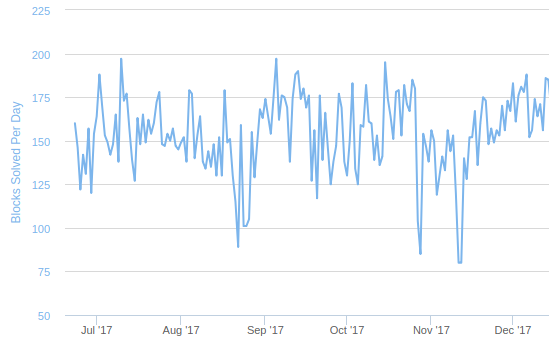
\includegraphics[width=2.5in]{bitcoin1.png} \\
Bitcoin blocks per day \\
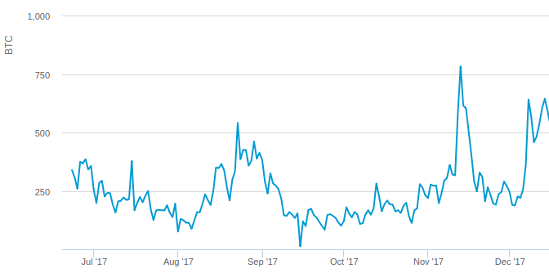
\includegraphics[width=2.5in]{bitcoin2.png} \\
Bitcoin transaction fees
\label{fig:three}
%\end{figure}
\end{center}

A more thorough analysis of similar data\cite{demand-elasticity} gives elasticities of 0.4-0.7 for Bitcoin, and 1-2 for Ethereum.

Additionally, it is important to note that this only measures the short-term demand curve looking at actions taken over a few days to months and does not take into account longer-term adjustments that could happen in the market only after a couple of years; in the real world, for example, it is an established fact that long-run demand elasticity of gasoline is higher than short-run elasticity\cite{env-econ}; and this is likely true with Bitcoin transaction fees and Ethereum gas as well.

So far, this model suggests a benefit curve with slope between -0.4 and -2 (if rescaled so that the current supply/demand intersection is at $(1, 1)$), and a social cost curve with (rescaled) slope that is difficult to determine, but at current margins in various blockchains is likely to be low and may be positive or negative. This suggests that a flat per-weight-unit in-protocol transaction fee, coupled with a hard limit at the point where the marginal social cost starts rapidly increasing, is superior to a pure weight limit-based regime.

------------------

\section{Cryptocurrency Prices}

In the short run, one can assume that price movements, changes in the social cost functions and changes in usage are all random and independent. In the long run, however, the three factors are highly intertwined. Specifically, (i) the price of a cryptocurrency; (ii) the social cost curve [as the number of beneficiaries of the system increases, and the number of full nodes also increases]; and (iii) the benefit curve [as there are more users sending transactions] are all highly correlated with a single variable, which we might call ``adoption''.

We can make a model as follows. Suppose that a k-factor increase in adoption leads to:

\begin{itemize}
    \item A k-factor increase in the price.
    \item A k-factor increase in the number of transaction users, ie. a k-factor horizontal stretch of the demand curve.
    \item A k-factor increase in the number of users and the number of full nodes.
\end{itemize}

Let us assume for simplicity that the demand elasticity is 1, and that the decentralization utility of $N$ full nodes is $D(N) = \log(N)$, so a k-factor increase in the number of full nodes simply adds utility $\log(k)$; the k-factor increase in the number of users scales up the social cost curve by a factor of k, and the private benefit curve scales by a factor of $k$. This leads to the result that, denominated in the cryptocurrency in question, adoption leaves the private benefit and social cost curves unchanged, and so there is also no correlation (!!). \footnote{An astute reader might ask whether or not there is empirical data to support this claim; unfortunately, far less than a single cryptocurrency ``business cycle'' (in the financial market bubble sense) has passed since blockchains started to typically have ``full blocks'', so there is far too little empirical data to make an assessment.}

Reality is of course more complicated than this simple model, but the model does suffice to show that, because of the lucky coincidence of being forced to denominate fees in a cryptocurrency whose price is itself proportional to adoption, there is at least no very strong first-order reason to expect positive correlation between the nominal benefit and cost curves. Hence, the arguments for using fixed fees in addition to gas limits still stand.

Arguably one of the key reasons behind the un-intuitiveness of fixed fees is that for most of the history of blockchain protocols, blockchains operated in a ``non-full blocks'' mode, where there was always space in a block to include more transactions. The fee required to be paid was only a minimal value, set as a software default. When a cryptocurrency experiences a large price rise, this causes fees experienced by users to rise greatly, until eventually the defaults are manually adjusted downwards \cite{coindesk-btc-txn-fee, reddit-rec-miners, vitalik-twitter1}.  Hence, transaction fees were kept artificially stable by what are essentially political constraints, whereas no such stabilizing effect existed for cryptocurrency prices.

\begin{center}
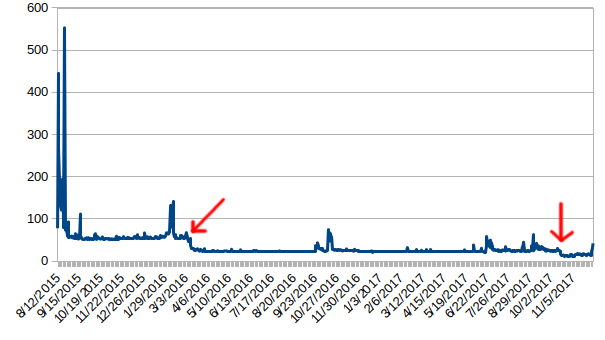
\includegraphics[width=3in]{GaspriceInGwei.png} \\
\scriptsize{Gas prices in gwei. The two marked sudden drops are coordinated attempts by miners and developers to reduce minimum accepted gasprices, first from 50 gwei to 20 gwei, then from 20 gwei to 4 gwei. Similar coordinated fee decreases have taken place in Bitcoin\cite{btcfeesdown10x}.}
\end{center}

However, Bitcoin has recently entered the ``full blocks'' regime, where transactions are in permanent competition with each other to get included, and Ethereum has entered this regime during high-intensity token sales\cite{braveICO}. In this mode, fees become more volatile, and rises in adoption contribute to even more volatility. In Bitcoin, this has led to a $\sim 10x$ increase in fees in less than a year; in Ethereum, fees increase by a similar factor during token sales. Even on average, in the last year transaction fees have become considerably more volatile than the ETH price:

\begin{center}
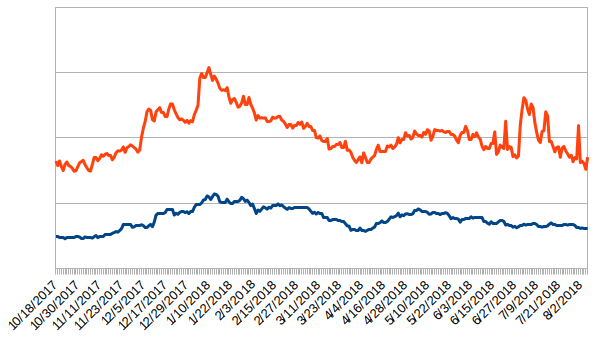
\includegraphics[width=3in]{PriceAndFees.png} \\
\scriptsize{ETH price (lower) and average gasprice in USD (higher), Oct 2017 (post-Byzantium-hardfork) to July 2018. The mean absolute daily percentage change is 4.2\% for the ETH price in the shown time period, and 16.0\% for the USD-denominated average gasprice, and is standard deviation is used the average gasprice is $\approx 25$ times more volatile due to spikes.}

\footnote{Source: http://etherscan.io/charts; spreadsheet with data and calculations at http://vitalik.ca/files/FeesAndETH.ods}
\end{center}

In the absence of political pressure on miners to make further gas limit increases, we see no reason for this state of affairs not to continue; and if political pressure \emph{can} be used to increase gas limits when needed, then the same processes could be used to adjust a fixed dee.

\section{Transaction Fees and Auction Theory}

So far, we have discussed resource pricing policies in the abstract, but we have not discussed the specific \emph{mechanism} that is used to implement them. The field of mechanism design has made many discoveries about what types of auctions perform better under what circumstances, and much of it is relevant to transaction fee markets.

In nearly all blockchains so far, transaction fee markets work as follows. Transaction senders are free to specify any fee they want as part of their transaction when they broadcast it. Transactions are included into blocks by \emph{block proposers}, which we can assume here are randomly selected for each block. Block proposers are constrained by the weight limit, which specifies how much they can include in each block. Naturally, block proposers will include the transactions that pay them the most, and as part of the protocol they collect the fees that are specified in the transaction.

In mechanism design speak, this is a \emph{first price auction}, characterized by the key property that ``you pay what you specify, and only if you win''. This kind of auction is generally considered to be deeply suboptimal, because it requires complex and inefficient strategies on the part of the buyers (here, transaction senders). For example, suppose that a given buyer values their transaction getting included at \$1. How much should they bid? The answer is certainly less than \$1; but how much less? If everyone else is bidding \$0.05, then clearly \$0.06 will suffice. If everyone else is bidding fees that have some complex distribution with mean \$0.10 and standard deviation \$0.05, with a fat tail on the right side, then the calculation becomes extremely complicated, and very often there are no efficient equilibria. \cite{poa-in-auctions} \footnote{The inefficiency of first price auctions in existing blockchain networks has already shown itself with many cases of users and businesses overpaying for fees \cite{bithumb-fees}, and self-help articles directing users to tools that facilitate ``fee estimation''\cite{fee-estimation}.}

The typical alternative is for selling many items a \emph{kth price auction}: everyone pays the same as the lowest fee that gets included. \footnote{Technically, everyone should pay the same as the highest fee that did \emph{not} get included, but this is even harder to implement and enforce, and for a sufficiently large number of items the difference between the two is very minor.} This mechanism allows for a very simple, and optimal, buyer-side strategy: if a transaction sender values getting their transaction included at \$x, they bid \$x. If the minimum bid in a block ends up being less than \$x, they get in (and pay less than \$x, so they are happy that they got in), but their bid being higher does not marginally affect the \emph{amount} they pay. If the minimum bid in a block ends up being more than \$x, the transaction sender does not get included, and is happy they were not included, because were they included they would have had to pay a fee higher than they were willing to pay.

However, kth price auctions have a different kind of serious flaw: they are not incentive-compatible \emph{for the auctioneer} (ie. the block proposer). First of all, if a block proposer is presented with a suitably steep demand curve, it is in their interest to fill the block with at least some high-fee-paying ``dummy transactions'', displacing low-fee-paying transactions and sacrificing the revenue from these transactions but at the same time dramatically raising the fee that \emph{everyone else} has to pay.

\begin{center}
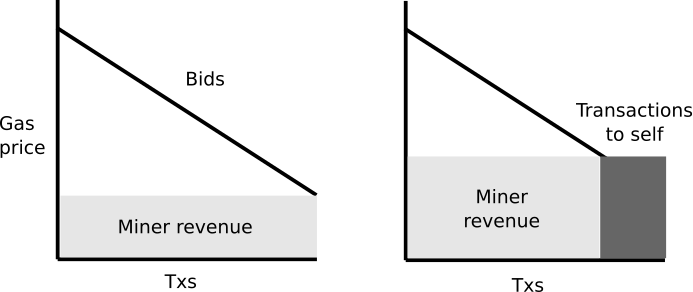
\includegraphics[width=3.5in]{kth_price_revenue.png} \\
\end{center}

A more serious issue is \emph{collusion} between the proposer and some transaction senders. A proposer can potentially collude with low-fee tansaction senders (eg. suppose there is a single entity, like an exchange or mining pool, that sends such transactions and can b easily negotiated with) that are sending transactions with some fee $f_{low}$. The proposer can ask them to instead send their transactions with fee $f_{high}$, and refund them $f_{high} - \frac{f_{low}}{2}$. The proposer's revenue is now even higher: the proposer benefits from the increased height of the ``rectangle'' of fee revenue that they would get with the ``dummy transaction'' strategy above, but they would also get a portion of the revenue from transactions that they would otherwise have sacrificed. \footnote{For a more detailed treatment of similar issues, see \cite{li2018} and \cite{rothkopf2007}.}

Hence, both first-price and second-price auctions are unsatisfactory. However, note that these issues are exclusively properties of auctions, and not properties of a fixed-price sale. If being included in the blockchain simply requires paying some $minFee$, then transaction senders have a simple strategy that they can use to set the fee on their transaction. Let $v$ be a user's private valuation for a transaction getting included in the next block. The user would check if $v > minFee$; if it is, they would bid $minFee + \epsilon$ (to provide a slight incentive for the block producer to include the transaction); if $v < minFee$ they would not send the transaction. This is a very simple strategy that does not require knowledge of others' valuations, and is optimal for the transaction sender.

\section{Improving the Second Best}

So far the evidence suggests that hard quantity limits are overused and price floors are underused. But how do we even start trying to set the price floor? What we will show in this section is that in cases where a price floor is better, it is possible to improve upon a hard quantity limit in a way that specifically alleviates the problem of deadweight losses from \emph{short-term transaction fee volatility}, without having to set a specific price as a protocol parameter. Clearly, large deadweight losses from short-term transaction fee volatility exist: Ethereum transaction fees are sometimes 2 gwei and sometimes 100 gwei, but it is definitely not true that the marginal social cost of a block containing 8000001 gwei rather than 8000000 is 50 times higher in the case where the latter is true.

Suppose that we start with an existing policy which sets a weight limit $w_{max}$. We normalize weight units so that the \emph{optimal} weight limit and transaction fee level are both 1. For simplicity, we assume linearity of the marginal social cost and demand function: $C'(1 + x) = 1 + C'' * x$ and $D'(1 + x) = 1 - D'' * x$, where $D''$ can also be viewed as the demand elasticity. Suppose that $w_{max}$ is set incorrectly, to $1 + r$ for some $r$ (in reality, $w_{max}$ will of course inevitably be set incorrectly, though we likely won't know the value of $r$ or even if it is positive or negative). We can draw a deadweight loss triangle to calculate the size of the economic inefficiency:

\begin{center}
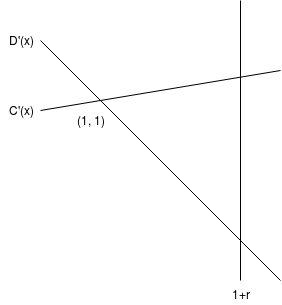
\includegraphics[width=2.5in]{Triangle1.png} \\
\end{center}

The area of the triangle, representing the total economic losses from an excessive (or if $r$ is negative, insufficient) number of transactions being included, is $\frac{1}{2} * r^2 * (C'' + D'')$; for simplicity we'll call this value $A$. Now suppose that, like in reality, demand is volatile, which we will approximate with a simple model where $D'(1 + x)$ half the time equals to $1 + D'' * x + \delta$ and the other half of the time equals to $1 + D'' * x - \delta$. In the $-\delta$ period, the height of the triangle increases from $r * (C'' + D'')$ to $r * (C'' + D'') + \delta$, or a ratio of $1 + \frac{\delta}{r * (C'' + D'')}$.

\begin{center}

\includegraphics[width=2.5in]{Triangle2.png} \\
\end{center}

By similar triangle laws the width increases by the same proportion, so the area increases from $A$ to $A * (1 + \frac{\delta}{r * (C'' + D'')})^2$. In the $+\delta$ period, the area decreases to $A * (1 - \frac{\delta}{r * (C'' + D'')})^2$. The average of $(1+x)^2 + (1-x)^2$ is $1 + x^2$, so the average of the two areas is $A * (1 + (\frac{\delta}{r * (C'' + D'')})^2)$.

Now, suppose we use a different algorithm. The protocol targets a \emph{long run} average weight of $1 + r$, but it does so by setting a price for transactions that adjusts slowly over time. The price that it would target is in this case is $1 - D'' * r$. Now, let us consider the average deadweight loss. Moving demand up by $\delta$ will move the triangle to the right by $\frac{\delta}{D''}$, which increases its height by $\frac{\delta * C''}{D''}$.

\begin{center}

\includegraphics[width=2.5in]{Triangle3.png} \\
\end{center}

The original height was $r * (C'' + D'')$, so the height increases by a ratio of $1 + \frac{\frac{\delta * C''}{D''}}{r * (C'' + D'')}$. By similar triangle laws the width increases by the same proportion, and in the $-\delta$ case we flip the sign in a similar way; the end result is that the average area is $A * (1 + (\frac{\frac{\delta * C''}{D''}}{r * (C'' + D'')})^2)$.

It should be clear that the average area in the second case is smaller (ie. less inefficiency) than the average area in the first case if and only if $\frac{\frac{\delta * C''}{D''}}{r * (C'' + D'')} < \frac{\delta}{r * (C'' + D'')}$, or alternatively $\frac{\delta * C''}{D''} < \delta$, or even more simply $C'' < D''$, and in other cases the average area in the second case is larger. What this thus proves is a sort of marginal analogue to Weitzman's 1974 result \cite{weitzman1974prices}, where in the exact same case where choosing a price is better than choosing a quantity, a quantity limit can be improved on the margin by replacing it with a ``flexible limit'' that is really just a price level that adjusts over the medium term to target the quantity limit.

We now propose an alternate resource pricing/limit rule that we believe provides superior properties to a hard limit $w_{max}$:

\begin{itemize}
\item Define a constantly adjusting in-protocol parameter $minFee$. Transaction senders are charged a fee of $minFee$ per weight unit; this fee is either burned or redistributed to consensus participants \emph{other than} the proposer of the block that included this transaction; this prevents profitable side-dealing arrangements where the transaction senders are refunded this fee.
\item Define a new weight limit, $w_{newmax} = 2 * w_{max}$.
\item Define an \emph{adjustment speed parameter} $adjSpeed$, with $0 < adjSpeed < 2$.
\item In any particular block, let $w_{prev}$ be the amount of weight consumed in the previous block, and $minFee_{prev}$ be the previous block's $minFee$ value. See $minFee$ for this block to equal $minFee_{prev} * (1 + (\frac{w_{prev}}{w_{newmax}} - \frac{1}{2}) * adjSpeed$.
\end{itemize}

This rule is likely to outperform simple limits in terms of allocative efficiency for the reasons cited above, and also (except during sudden and extreme spikes) eliminates the issues with first and second price auctions described above. \footnote{In the specific case of storage pricing, a quirk in Ethereum gas pricing rules that allows storage to be (mostly) paid for before it is actually used allows for second-layer markets like GasToken\cite{gastoken} where gas can be burned to generate ``congealed storage use privileges'', which can then be used later. The possibility of doing this unintentionally creates efficiency gains similar to those described here.}

As a philosophical note, complex gas and fee policies are often criticized as being a form of economic ``central planning'', which is frowned upon because planners may not have aligned incentives and have less information than participants closer to the day-to-day economic activity. That said, note that \emph{any} transaction pricing policy, whether fee-based or limit-based, necessarily has centrally planned parameters. I would argue that the correct way to apply the Hayekian anti-central-planning intuition is to treat it as saying that central plans are less bad if those plans have \emph{lower Kolmogorov complexity}, a simple strict weight limit being an ideal example.

Plans with low Kolmogorov complexity are ideal because they have fewer moving parts that can fail, are less likely to overfit, and because there is so little entropy in the specification and parametrization of the plan, it is very difficult to encode attempts to favor or disfavor specific users or applications; this helps foster a shared impression of fairness. For this reason, we will argue for policies that are as simple as possible while still being substantial and needed improvements on the status quo.

\section{Heterogenous Resources in Computation and Bandwidth}

The above weight limit analyses assume that a single scalar can sufficiently quantify the burden a transaction imposes upon the network. In reality, however, a transaction consumes several heterogeneous resources: calculation and state I/O (here grouped into ``computation''), bandwidth, and state storage.  Each of these have different properties, and an optimal pricing scheme should likely take these differences into account.

We will start off by looking at computation and bandwidth. Computation and bandwidth both contribute to the computational load of a node, and both contribute to ``uncle rate''; hence, both seem to be subject to the same mechanics of linear or sublinear social cost at lower weights and superlinear social cost at higher weights. If the factors creating the superlinear social costs are independent, it may be prudent to have a separate gas limit for computation and block size limit for bandwidth; however, because much of the superlinearity comes from the uncle rate itself, and the impacts of computation and bandwidth on uncle rate seem to be additive, it seems more likely that a single combined limit actually is optimal.

One question worth asking is: can we somehow measure in-protocol the social cost of computation and bandwidth, or at least a more limited statistic like the maximum level of computation and bandwidth that the median client can safely handle? Proof of work mining difficulty does very directly give an exchange rate between a blockchain's native cryptocurrency and at least one kind of computation: if a blockchain's block reward is $R$, its mining algorithm is $H$, and its difficulty is $D$, then in general we should expect $cost(H) \approx \frac{R}{D}$.

However, this approach is extremely fragile against advances in technology such as specialized hardware. \cite{hardware1} and \cite{hardware2} suggest a roughly 1000-5000x difference between the mining efficiency of ASIC and GPU hardware for mining Bitcoin at present, and a further disparity exists between GPUs and CPUs. This suggests that, were mining difficulty used as a proxy to determine the computational capacity of clients in order to determine Bitcoin block size limits, a block size limit initially targeted to 1 MB would by now have grown to be many gigabytes. A block weight limit targeted to an optimal value based on the assumption of a 10000x disparity between ASICs and CPUs today may in contrast lead to the limit becoming 100-10000x \emph{below} optimal if the advantage of specialization \emph{decreases} in the future, due to either more use of adaptive semi-specialized hardware such as FPGAs in consumer hardware or specialized hardware being unable to squeeze out larger efficiencies once even general-purpose hardware starts to come close to thermodynamic limits.

The proof-of-work-based cost metric has an additional flaw: $cost(H)$ is only the cost of calculating a computation \emph{once}. The actual social cost also depends heavily on the number of nodes in the network, as each node will need to run the computation, and this is also extremely difficult to measure. This issue can be circumvented by changing the mechanism, instead requiring miners to compute a \emph{non-outsourceable} proof of work \cite{nonoutsourceable} and setting a computation gas limit based on the highest amount of work submitted within some time period, but this does not get around the specialized hardware issues. One can try to incentivize \emph{transaction submitters} to submit these proofs, but that carries the high risk of incentivizing users to use wallets with centralized custody of private keys.

One can similarly attempt to measure bandwidth with proofs of bandwidth \cite{proof-of-bandwidth}, but this also carries a high risk of incentivizing concentration. Fundamentally, incentive-compatibly measuring the level of capability of a node requires incentivizing them to reveal capability, with higher rewards for higher levels of revealed capability, and this inherently incentivizes specialized and concentrated hardware-driven centralization.

\section{Pricing State Storage}
\label{sect:storage}

Pricing state storage is a fundamentally different kind of burden from computation, bandwidth and state IO (treated above as being simply another kind of computation) for one simple reason: whereas those costs are one-time burdens on validators and nodes that are online at that particular time, state space must be stored by, and thus burdens, all full nodes, forever.

In Bitcoin, there is no explicit fee for filling storage; transactions are simply charged per byte, and filling storage is charged for indirectly because filling a new storage slot (consuming an average 61 bytes\cite{utxo1}) requires adding about 34 bytes\cite{utxo2} to a transaction (at least for ``regular'' outputs; non-standard outputs can be made for as little as 9 bytes\cite{utxo3}\cite{utxo4}), so there is a maximum amount by which one can increase the size of the UTXO set within a single block. The recent Segregated Witness fork includes a modification where signature data is charged as 1 weight unit per byte and nonsignature data as 4 weight units per byte, up to a maximum of 4 million weight units; this relatively reduces the cost of spending UTXOs and increases the cost of creating new UTXOs \cite{segwitwhy4}.

In Ethereum, there is a more complex gas cost schedule for storage-affecting operations, There are two types of operations that can affect the storage size:

\begin{enumerate}
    \item The \opcode{sstore} opcode, which saves a value in the contract's storage. If \opcode{sstore} overwrites an existing value, it costs 5000 gas, but if it adds a new value to storage, it costs 20,000 gas. If \opcode{sstore} is used to clear an existing value (so it no longer has to be saved in storage), then it costs the contract 5,000 gas, but a ``refund'' of 15,000 gas is given to the transaction sender.

    \item \emph{Account creation}. Accounts can be created\footnote{Accounts can also be deleted through the \opcode{selfdestruct} opcode, which costs the contract 5,000 gas but refunds the transaction sender a 24,000 gas.} in three ways:

    \begin{itemize}
        \item creating a contract using the \opcode{create} opcode (32,000 gas, plus 200 per byte of code)
        \item creating a contract using a transaction (53,000 gas, or 32,000 + the 21,000 base cost of sending a transaction)
        \item sending ether to a previously non-existent account (25,000 gas if done from a contract; if done from a transaction the 21,000 gas base cost).

    \end{itemize}

\end{enumerate}

The gas costs were computed by taking as a goal a cost of $\approx 200$ gas per byte in storage, estimating the number of bytes added to storage space by each particular type of storage-filling operation, multiplying the two values, and then adding an additional term to take into account other costs such as computation and contribution to history size.

However, both the Bitcoin and Ethereum approaches have four large problems that lead to very suboptimal outcomes:

\begin{itemize}
\item Storage is far too cheap in an absolute sense. For example, it costs 68 gas to force current users of the Ethereum network to download and process a byte, but 200 gas is enough to force all present and future users to do the same (and store the data forever)
\item The social cost of storage is far more linear, especially in the short and medium run, than computation, bandwidth and disk IO. If the storage normally increases by 1 MB per day, but in one month it increases by 100 kB per day most days except for the last day when it suddenly increases by 27 MB, the extra volatility in storage growth does not really hurt anyone.
\item There is insufficient incentive to clear storage. In the extreme case, depending on fee rates 10-60\% of the UTXOs in Bitcoin's state\cite{utxo5} have a value sufficiently low that it costs more money to clear them than is contained in the UTXOs. Most Ethereum contracts that get created do not get destroyed, and many do not have any effective ``storage hygiene''.
\item There is no incentive to clear storage earlier rather than later. Even if storage clearing refunds exist, at present they are not time-based.
\end{itemize}

The first problem can possibly be solved by simply making storage more expensive. However, making storage more expensive and doing nothing else would make it prohibitively expensive to use storage for very short periods of time. One could offer a time-based refund, refunding more if a storage slot is cleared earlier rather than later; the only arbitrage-free scheme for this is to define some decreasing nonnegative function $F(t)$ (eg. $F(t) = h * e^{-kt}$) of the current time, and charge $F(t)$ for filling a storage slot at time $t$, and refund $F(t)$ for clearing a storage slot at time $t$.\footnote{If different storage slots can have different $F(t)$ functions, then at any point where $F_1'(t) > F_2'(t)$, there is an arbitrage opportunity where if the holder of $F_1$ (the slower-falling function) no longer needs their storage slot, they can instead assign permission to use it to the holder of the other storage slot, and the holder of the other storage slot can clear it immediately.} However, this approach is very capital-inefficient, requiring large deposits to use storage, and additionally rests on the assumption that the social cost of storage will continue to forever decrease quickly enough that the integral is convergent.

A solution that does not have these problems is to implement a time-based storage maintenance fee (sometimes also called ``rent''). The simplest way to implement this is simple: every account object is charged X coins per block per byte that it consumes in the state. If an account has less coins than the amount needed to pay for $pokeThreshold$ blocks (say, $pokeThreshold = 500$), then anyone can ``poke'' the account and delete it from storage, and claim $k * pokeThreshold$ blocks' worth of rent as a bounty where $k \in (0,1]$. Implementing the above is impractical as every block going through every account and decrementing its balance has immense overhead. However, this can be computed quite practically through lazy evaluation:

\begin{itemize}
\item All accounts store an additional data field, $LastBlockAccessed$
\item An account's current balance can be computed as $$balance - perBlockFee * sizeOf(account) * (curBlock - LastBlockAccessed)$$
\item An account can be poked if this value goes below $perBlockFee * sizeOf(account) * pokeThreshold$
\item When an account's state is modified, its $balance$ is updated based on the above formula, and $LastBlockAccessed$ is set to the current block number
\end{itemize}

Suppose that we want the maintenance fee to be able to vary over time. Then, for all block heights $h$ we save in storage $totalFee[h] = \sum_{i=1}^h Fee[i] = totalFee[h-1] + Fee[h]$. We compute the current balance as $$balance - sizeOf(account) * (totalFee[curBlock] - totalFee[LastBlockAccessed])$$, where $totalFee[curBlock] - totalFee[LastBlockAccessed]$ can be understood as $\sum_{i=LastBlockAccessed}^{curBlock} Fee[i]$.

However, we will argue in favor of simply setting the maintenance fee to one specific value (eg. $10^{-7}$ ETH per byte per year), and leaving it this way forever. First of all, the social cost of storage use is clearly almost perfectly linear in the short and medium run, but it is also much more linear in the long run. There is no analog to the natural asymptote of bandwidth and computation costs in blockchains where at some point the uncle rate reaches 100\%; even if the storage of the Ethereum blockchain starts increasing by 10 GB per day, then blockchain nodes will be quickly relegated to only running on data centers, but the blockchain will still fundamentally be functional. In fact, if you assume that node storage capacity is distributed among the same distribution as the Cornell study\cite{cornell} shows bandwidth is, so $NodeCount(W) = \frac{1}{W}$, and assume the logarithmic utility function for node count, so $D(x) = log(x) = -log(W)$ then the social cost component from node centralization is roughly $C(W) = log(W)$, or $C'(W) = \frac{1}{W}$ - very steeply \emph{sublinear}.

Second, the developer and user experience considerably improves if developers and users can determine with exactness a minimum ``time to live'' for any given contract far ahead in advance. Variable fees do not have this property; a fixed fee does. Third, as cryptocurrency prices are more stable than transaction fees, a fixed fee improves price predictability, in both cryptocurrency and fiat-denominated terms. Fourth, a fixed fee is simple, both intuitively and in the semi-formal sense of having low Kolmogorov complexity.

\section{Storage Pricing and User Experience}

For a simple cryptocurrency, the harm from one particular UTXO or account being deleted because its balance was completely drained paying storage maintenance fees is very simple to understand, and there are no complex interaction effects between different accounts or UTXOs that could result. For a more complex smart contract blockchain, rent does introduce more complexities, as there will be contracts that are very valuable for reasons other than the ETH (or other protocol-level base currency) contained in them, such as their function as software libraries, user-defined assets (ERC20, ERC721, etc) that they hold, active relationships with other smart contracts, etc. Hence, there is larger risk of an application suddenly becoming unusable because someone forgot to pay a maintenance fee. 

Such situations can generally be detected far ahead of time, but if this happens, then there is a second backstop that can be added to mitigate the effect of deletions arising from negligent failure to pay maintenance fees: a \emph{hibernation/waking scheme}. Accounts that run out of funds to pay their maintenance fees do get removed from the state, but they are not \emph{deleted}; rather, they are \emph{hibernated}. For any hibernated contract, anyone can submit Merkle proofs that prove two claims:

\begin{enumerate}
\item A given hibernated contract exists.
\item That particular instance of hibernation was not already used to wake the contract.
\end{enumerate}

Condition (2) is needed to prevent a double-waking attack, where a contract is hibernated once, and then the proof of its hibernation is used to wake the old contract twice:

\begin{center}
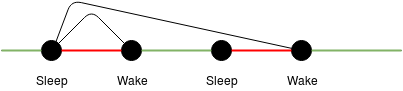
\includegraphics[width=3.5in]{sleepwake.png} \\
\end{center}

If the contract contains more funds at the time of the older hibernation that it does at the time of the newer hibernation, then such an attack could be used to create funds out of nowhere. The second kind of proof could be done as follows. Define $MinInterval$ as the minimum length of time a storage slot can be used for (eg. 1 week):

\begin{itemize}
\item Add a condition to the fee payment logic: when a contract is woken, it must be filled with at least $(MinInterval + pokeThreshold) * sizeOf(contract) * feePerBlock$ ether. A contract also cannot withdraw so much that its remaining balance after the withdrawal falls below this threshold.
\item A proof of non-prior-waking consists of a Merkle branch pointing to the contract's address once every $MinInterval$
\end{itemize}

Adjusting $MinInterval$ is a tradeoff: smaller values enable launching contracts cheaply for shorter periods of time, but larger values shrink the size of the witness required for waking, as well as shrinking the number of ever-growing historical state roots that need to be stored. For a $MinInterval$ of one week, and a state with $2^{30}$ accounts, waking a ten year old contract would require $32 * log(2<sup>30</sup>) * \frac{10 * 365.242}{7} \approx$ 500,000 bytes; a $minInterval$ of one month reduces this to 115,200 bytes.

\section{Conclusion}

Economic analysis can be used to significantly improve the incentive alignment of resource usage inside of public blockchains. Simplistic models of one-dimensional weight limits often lead to prices that are highly mismatched relative to social costs, and slightly more complex techniques involving a combination of ``Pigovian taxes'' and cap-and-trade mechanics such as weight limits can improve significantly on the status quo. Storage in particular is a very different resource market from other types of resource markets, and should be treated separately.

More economic analysis and econometric research can be used to help identify further mechanisms that can be used to better reduce costs while discouraging wasteful use of public blockchain resources.

\textbf{Acknowledgements.} \todo{fill me in.}


\bibliography{ethpricing}


\newpage
\appendix
\part*{Appendix}




%%%%%%%%%%%%%%%%%%%%%%%%%%%%%%%%%%%%%%%%%%%%%%%%%%%%%%%%%%%%%%%%%%%%%%%%%%%%%%%%%%%%%%%%%%%%%%
%% TABLES!
%%%%%%%%%%%%%%%%%%%%%%%%%%%%%%%%%%%%%%%%%%%%%%%%%%%%%%%%%%%%%%%%%%%%%%%%%%%%%%%%%%%%%%%%%%%%%%



%\begin{figure}
%\centering
%\subcaptionbox{Subcaption A}{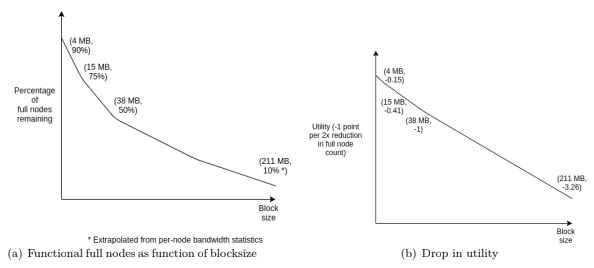
\includegraphics[width=3in]{blocksize_fullnodes.png} }%
%\hfill
%\subcaptionbox{Subcaption B}{ 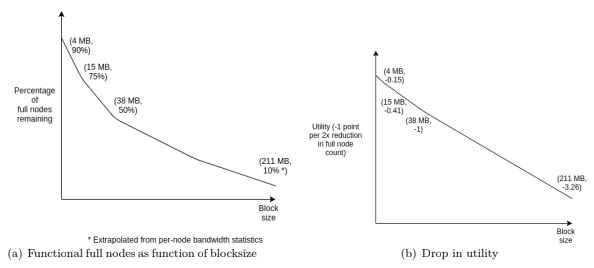
\includegraphics[width=3in]{blocksize_fullnodes.png} }%
%\caption{Caption}
%\end{figure}




\section{The Full Ethereum Gas Function}
\label{appendix:gasfunction}
\todo{Put the full gas function here.}


\end{document}
  
  
  
  
         

        
